% version 1.00, date 20/02/16, auteur Michel Cressant
Ce chapitre présente les maquettes pour chaque fonctionnalité.


\section{Fonctionnalité 1}
Ce paragraphe décrit les maquettes concernant la fonctionnalité 1. \\

La figure suivante (figure \ref{maquette1-1}) montre la maquette pour la création d'un profil.
\begin{figure}[H]
	\centering
	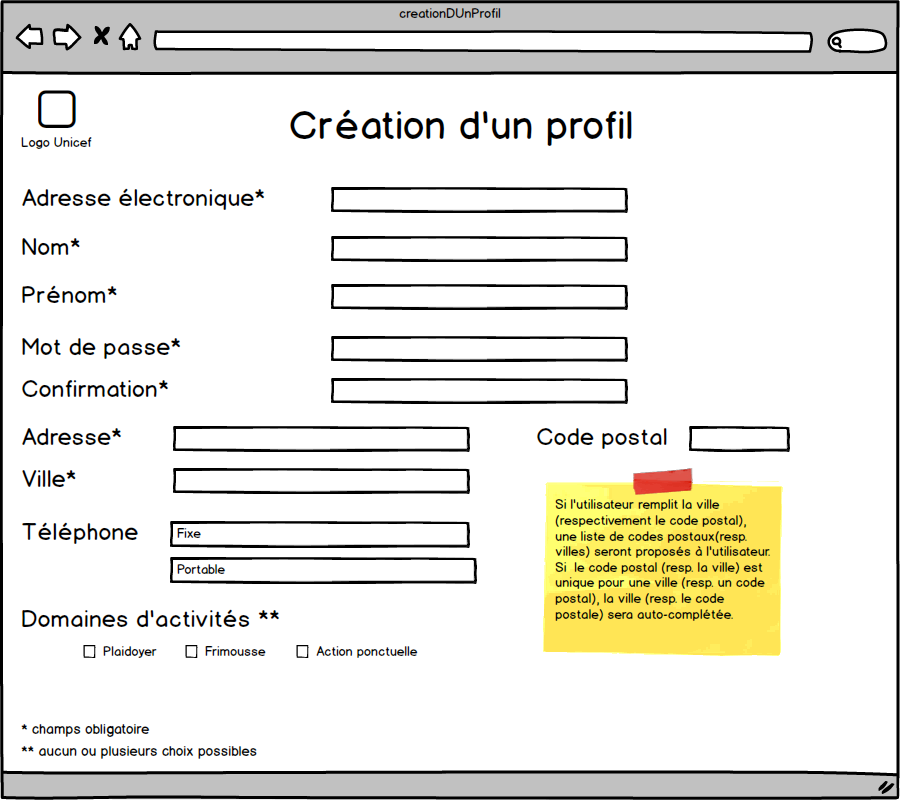
\includegraphics[scale=0.40]{images/maquettes/fonctionnalite1CreationDUnProfil.png}
	\caption{Maquette~: Création d'un profil }
	\label{maquette1-1}
\end{figure}

La figure suivante (figure \ref{maquette1-2}) montre la maquette pour la modification d'un profil.
\begin{figure}[H]
	\centering
	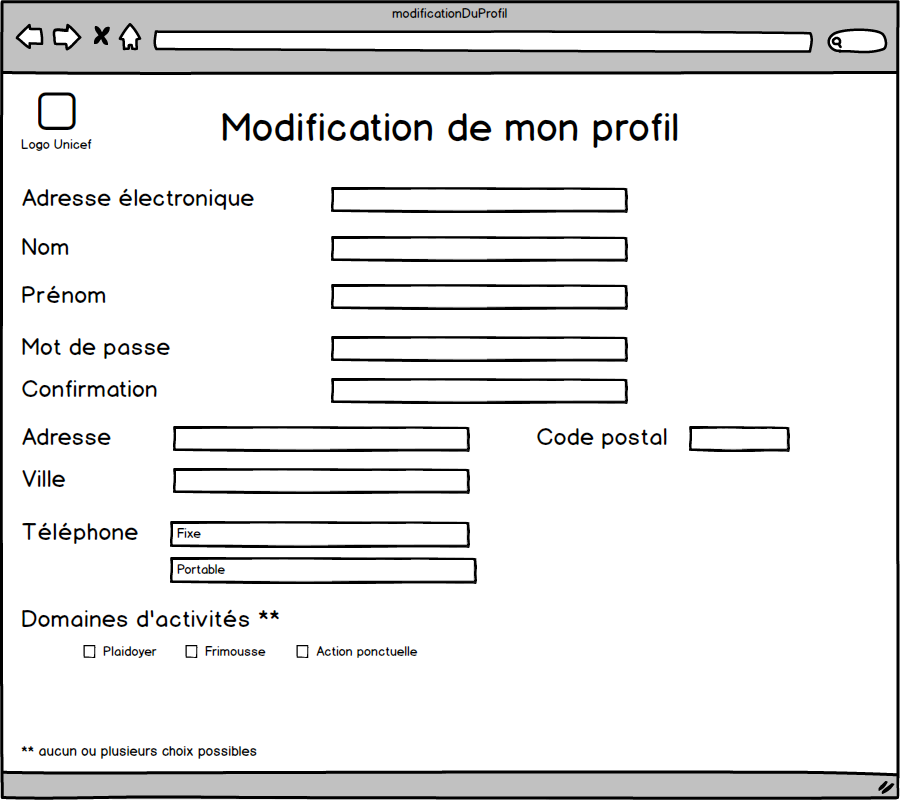
\includegraphics[scale=0.40]{images/maquettes/fonctionnalite1ModificationDUnProfil.png}
	\caption{Maquette~: Modification d'un profil}
	\label{maquette1-2}
\end{figure}

La figure suivante (figure \ref{maquette1-3}) montre la maquette pour la modification d'un profil par un administrateur.
\begin{figure}[H]
	\centering
	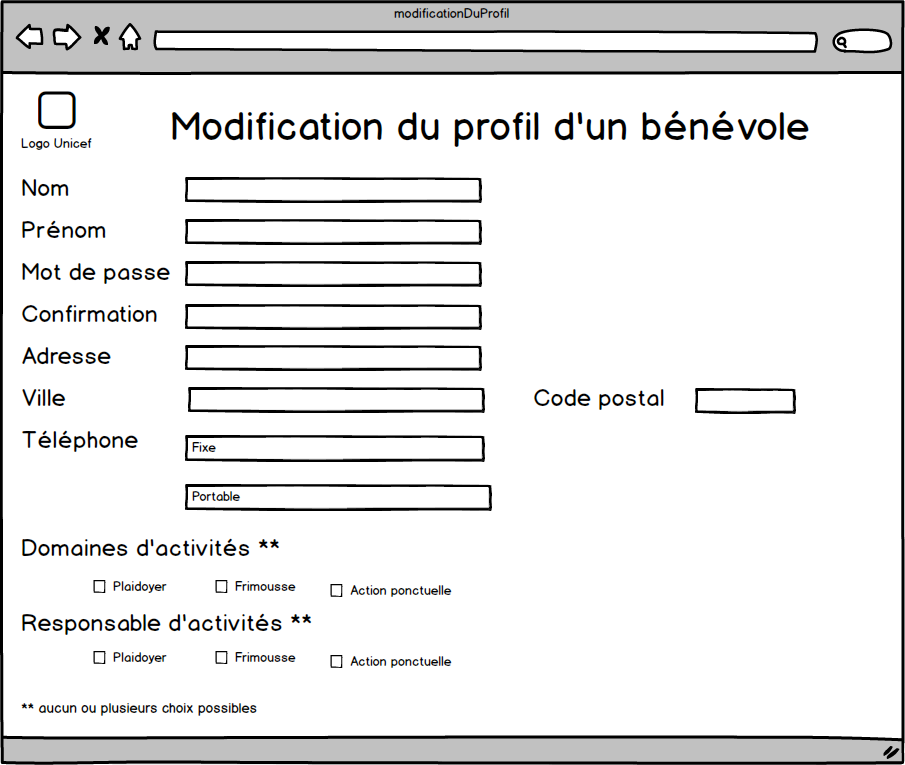
\includegraphics[scale=0.5]{images/maquettes/fonctionnalite1ModificationDUnProfilAdmin.png}
	\caption{Maquette~: Modification profil par un administrateur}
	\label{maquette1-3}
\end{figure}

\section{Fonctionnalité 3}
Ce paragraphe décrit la maquette concernant la fonctionnalité 3. \\

La figure suivante (figure \ref{maquette3-1}) montre la maquette pour le formulaire de demande d'intervention.
\begin{figure}[H]
	\centering
	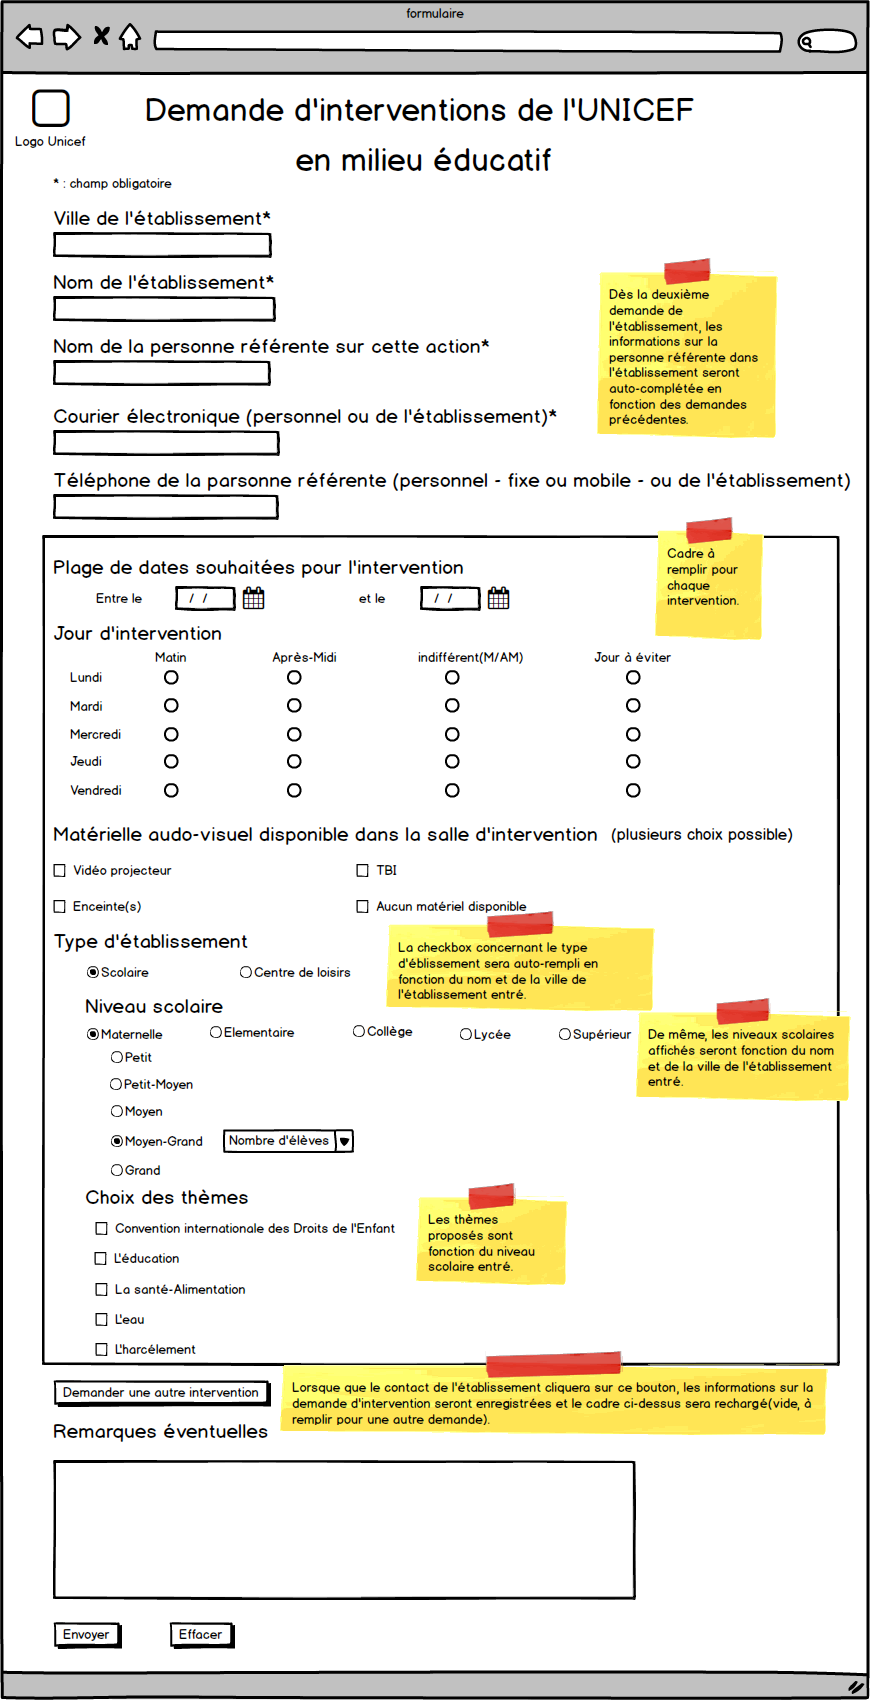
\includegraphics[scale=0.3]{images/maquettes/fonctionnalite3FormulaireDeDemandeDInterventions.png}
	\caption{Maquette~: Formulaire de demande d'intervention}
	\label{maquette3-1}
\end{figure}

La figure suivante (figure \ref{maquette3-2}) montre l'email type de demande d'intervention aux établissements.
\begin{figure}[H]
	\centering
	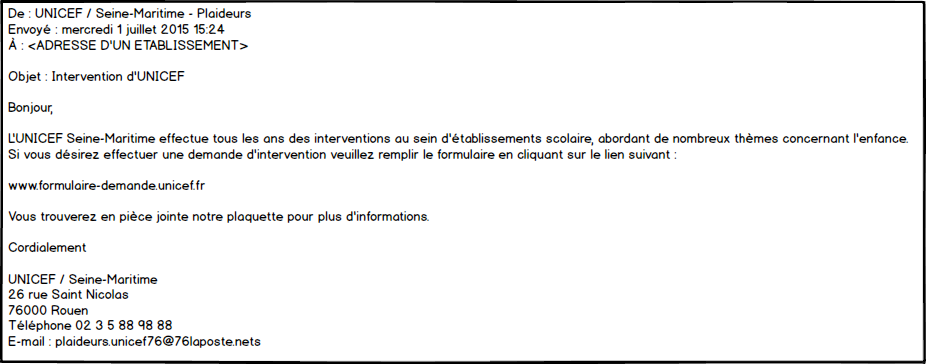
\includegraphics[scale=0.3]{images/maquettes/fonctionnalite3MailType.png}
	\caption{Maquette~: Email type de demande d'intervention}
	\label{maquette3-2}
\end{figure}

\section{Fonctionnalité 4}
Ce paragraphe décrit la maquette concernant la fonctionnalité 4. \\

La figure suivante (figure \ref{maquette4-1}) montre l'email type de confirmation de réception de demande.
\begin{figure}[H]
	\centering
	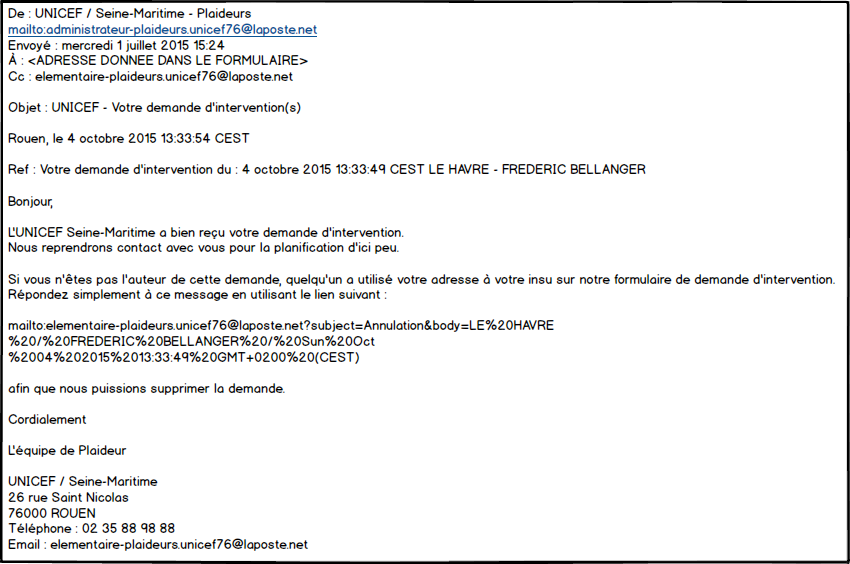
\includegraphics[scale=0.4]{images/maquettes/fonctionnalite4MailConfirmationReceptionDemande.png}
	\caption{Maquette~: Email type de confirmation réception de demande}
	\label{maquette4-1}
\end{figure}

La figure suivante (figure \ref{maquette4-2}) montre l'email type pour l'administrateur de confirmation de suppression d'une demande.
\begin{figure}[H]
	\centering
	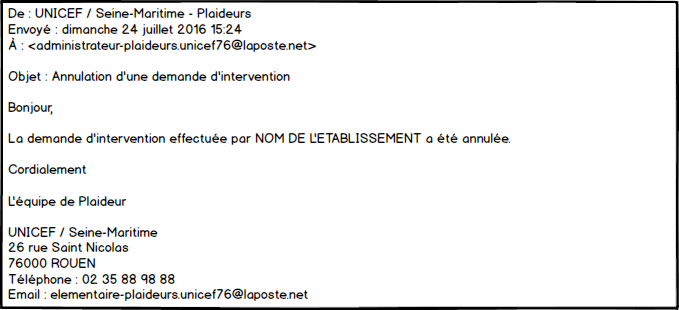
\includegraphics[scale=0.4]{images/maquettes/fonctionnalite4MailConfirmationSuppressionDemandePourAdmin.png}
	\caption{Maquette~: Email type administrateur de confirmation suppression de demande}
	\label{maquette4-2}
\end{figure}

La figure suivante (figure \ref{maquette4-3}) montre l'email type pour l'établissement de confirmation de suppression d'une demande.
\begin{figure}[H]
	\centering
	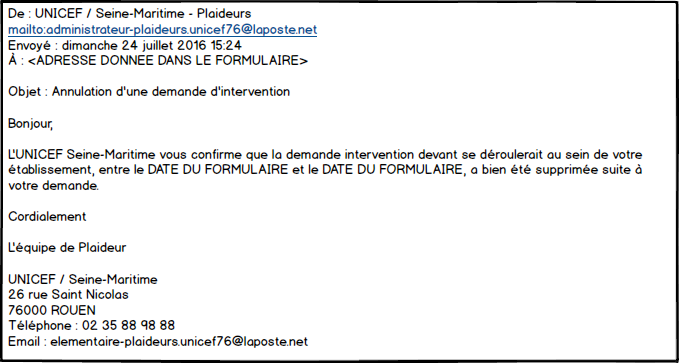
\includegraphics[scale=0.4]{images/maquettes/fonctionnalite4MailConfirmationSuppressionDemandePourEtablissement.png}
	\caption{Maquette~: Email type établissement de confirmation suppression de demande}
	\label{maquette4-3}
\end{figure}

\section{Fonctionnalité 5}
Ce paragraphe décrit la maquette concernant la fonctionnalité 5. \\

La figure suivante (figure \ref{maquette5-1}) montre la maquette de la géolocalisation des interventions ainsi que l'affectation d'un plaideur à celles ci. \\
\begin{figure}[H]
	\centering
	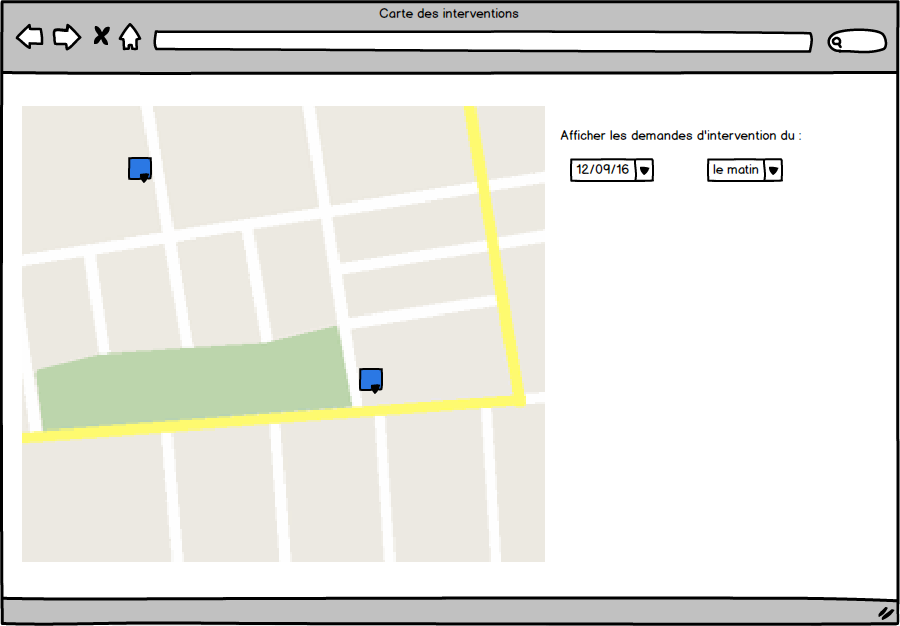
\includegraphics[scale=0.35]{images/maquettes/fonctionnalite5CarteDesInterventions.png}
	\caption{Maquette~: Géolocalisation des interventions et affectation à une intervention}
	\label{maquette5-1}
\end{figure}

La figure suivante (figure \ref{maquette5-2}) montre l'email type de prise en charge. \\
\begin{figure}[H]
	\centering
	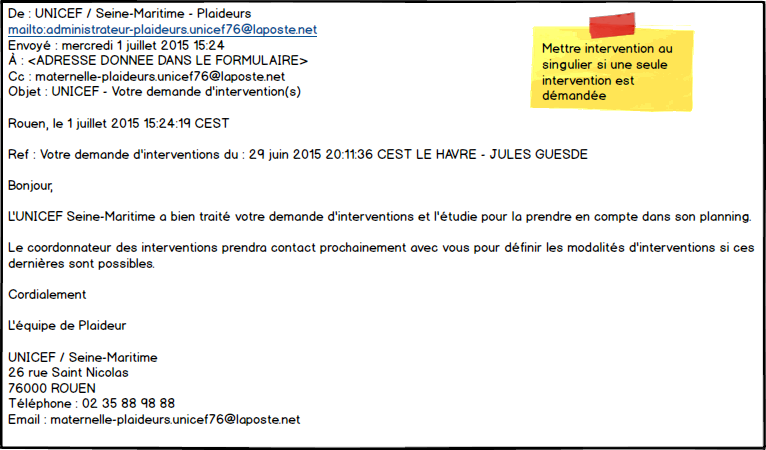
\includegraphics[scale=0.35]{images/maquettes/fonctionnalite5MailDePriseEnCharge.png}
	\caption{Maquette~: Email type de prise en charge}
	\label{maquette5-2}
\end{figure}


\section{Fonctionnalité 6}
Ce paragraphe décrit la maquette concernant la fonctionnalité 6. \\

La figure suivante (figure \ref{maquette6}) montre l'email type récapitulatif des informations d'une intervention pour l'établissement.
\begin{figure}[H]
	\centering
	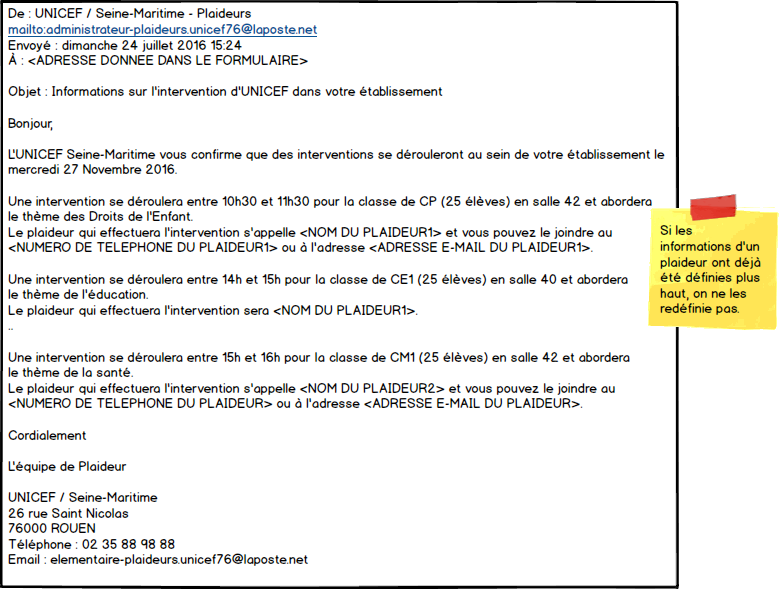
\includegraphics[scale=0.4]{images/maquettes/fonctionnalite6MailDInformationPourLEtablissement.png}
	\caption{Maquette~: Email type récapitulatif des informations d'une intervention pour l'établissement}
	\label{maquette6}
\end{figure}




\section{Fonctionnalité 7}
Ce paragraphe décrit la maquette concernant la fonctionnalité 7.\\

La figure suivante (figure \ref{maquette7}) montre l'email type de rappel pour le plaideur.
\begin{figure}[H]
	\centering
	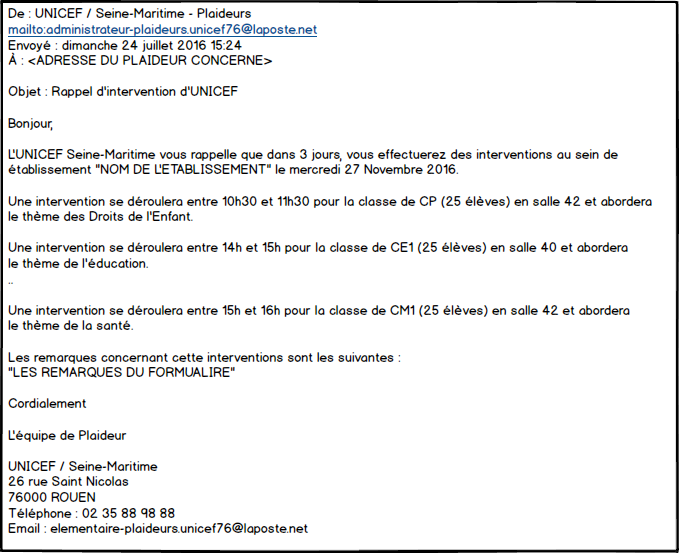
\includegraphics[scale=0.4]{images/maquettes/fonctionnalite7MailDeRappelPourLePlaideur.png}
	\caption{Maquette~: Email type de rappel pour le plaideur}
	\label{maquette7}
\end{figure}

La figure suivante (figure \ref{maquette7}) montre l'email type de rappel pour l'établissement.
\begin{figure}[H]
	\centering
	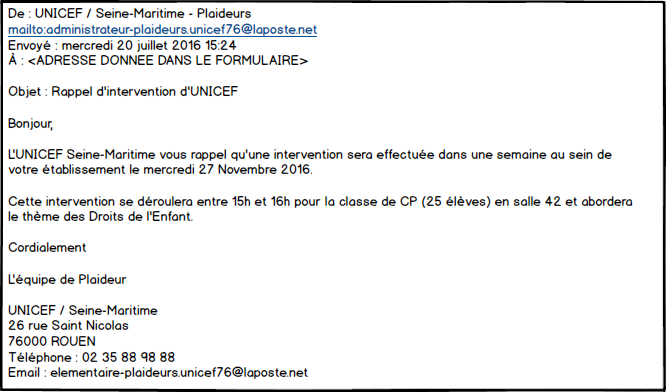
\includegraphics[scale=0.4]{images/maquettes/fonctionnalite7MailDeRappelPourLEtablissement.png}
	\caption{Maquette~: Email type de rappel pour l'établissement}
	\label{maquette7}
\end{figure}
